\documentclass[11pt]{article}

% ==== Paquetes ====
\usepackage[utf8]{inputenc}
\usepackage[spanish]{babel}
\usepackage[T1]{fontenc}
\usepackage{amsmath, amssymb, amsfonts, siunitx}
\usepackage{graphicx}
\usepackage{float}
\usepackage{xcolor}
\usepackage{hyperref}
\usepackage{caption}
\usepackage{subcaption}
\usepackage{geometry}
\usepackage{listings}
\usepackage{tikz}

\definecolor{codegreen}{rgb}{0,0.6,0}
\definecolor{codegray}{rgb}{0.5,0.5,0.5}
\definecolor{codepurple}{rgb}{0.58,0,0.82}
\definecolor{backcolour}{rgb}{0.95,0.95,0.92}

\lstset{
  inputencoding=utf8,
  extendedchars=true,
  literate=
   {á}{{\'a}}1 {é}{{\'e}}1 {í}{{\'i}}1 {ó}{{\'o}}1 {ú}{{\'u}}1
   {Á}{{\'A}}1 {É}{{\'E}}1 {Í}{{\'I}}1 {Ó}{{\'O}}1 {Ú}{{\'U}}1
   {ñ}{{\~n}}1 {Ñ}{{\~N}}1
   {¿}{{?`} }1 {¡}{{!`} }1
}

\lstdefinestyle{mystyle}{
    backgroundcolor=\color{backcolour},   
    commentstyle=\color{codegreen},
    keywordstyle=\color{magenta},
    numberstyle=\tiny\color{codegray},
    stringstyle=\color{codepurple},
    basicstyle=\ttfamily\footnotesize,
    breakatwhitespace=false,         
    breaklines=true,                 
    captionpos=b,                    
    keepspaces=true,                 
    numbers=left,                    
    numbersep=5pt,                  
    showspaces=false,                
    showstringspaces=false,
    showtabs=false,                  
    tabsize=2,
    upquote=true,
    inputencoding=utf8,
}

\lstset{style=mystyle}

\geometry{margin=2.5cm}

% ==== Datos de la tarea ====
\title{IEE3584 - Comunicaciones inalámbricas \\
Tarea 5}
\author{Nicolás Seguel}
\date{Septiembre 2025}

\begin{document}
\maketitle

\section*{Problema 19:}

\subsection*{a) Determine los valores óptimos de las ganancias $\hat{u}_r^*$ de cada rama transmisora.}

Se tiene que la ganancia óptima de cada rama transmisora está dada por:

\[
\hat{u}_r^* = \frac{h_r^*}{\sqrt{\sum_{k=1}^{N_R} |h_k|^2}}
\]

Para los datos dados en el problema, se tiene:

\begin{align*}
    N_r &= 18 \\
    \bar{\gamma} &= 17.8 \, \text{dB} \\
\end{align*}

Calculando las ganancias óptimas se tiene que:

\begin{align*}
    \hat{u}_1^* &= -0.06196161+0.22209773j  \\
    \hat{u}_2^* &= 0.19389928+0.40663906j \\
    \hat{u}_3^* &= -0.19430098+0.10495965j \\
    \hat{u}_4^* &= 0.08395365+0.13052314j \\
    \hat{u}_5^* &= 0.06558394+0.16405156j \\
    \hat{u}_6^* &= -0.24175322+0.20392136j \\
    \hat{u}_7^* &= -0.13829162+0.01330206j \\
    \hat{u}_8^* &= -0.1930639 -0.00873579j \\
    \hat{u}_9^* &= -0.12556898+0.13723031j \\
    \hat{u}_{10}^* &= 0.07308631+0.1780247j \\
    \hat{u}_{11}^* &= -0.00237966-0.1104075j \\
    \hat{u}_{12}^* &= -0.1040827 +0.00208126j \\
    \hat{u}_{13}^* &= -0.03603494-0.04405181j \\
    \hat{u}_{14}^* &= -0.40585926+0.21458815j \\
    \hat{u}_{15}^* &= -0.01591905+0.16429076j \\
    \hat{u}_{16}^* &= 0.12944699-0.31731982j \\
    \hat{u}_{17}^* &= -0.08245018+0.09513532j \\
    \hat{u}_{18}^* &= 0.07028502+0.09473617j
\end{align*}

\subsection*{b) Determine la razón señal a ruido de cada rama y la razón señal a ruido en la salida del combinador, en decibeles.}

La razón señal a ruido (SNR) de cada rama está dada por:

\[
\gamma_r = \bar{\gamma} |h_r|^2
\]

Calculando la SNR de cada rama se tiene:

\begin{align*}
    \gamma_1 &= 13.9134 \, \text{dB} \\
    \gamma_2 &= 53.1116 \, \text{dB} \\
    \gamma_3 &= 12.7627 \, \text{dB} \\
    \gamma_4 &= 6.3027 \, \text{dB} \\
    \gamma_5 &= 8.1685 \, \text{dB} \\
    \gamma_6 &= 26.1770 \, \text{dB} \\
    \gamma_7 &= 5.0511 \, \text{dB} \\
    \gamma_8 &= 9.7743 \, \text{dB} \\
    \gamma_9 &= 9.0545 \, \text{dB} \\
    \gamma_{10} &= 9.6917 \, \text{dB} \\
    \gamma_{11} &= 3.1914 \, \text{dB} \\
    \gamma_{12} &= 2.8361 \, \text{dB} \\
    \gamma_{13} &= 0.8476  \, \text{dB} \\
    \gamma_{14} &= 55.1574 \, \text{dB} \\
    \gamma_{15} &= 7.1298 \, \text{dB} \\
    \gamma_{16} &= 30.7356 \, \text{dB} \\ 
    \gamma_{17} &= 4.1475 \, \text{dB} \\ 
    \gamma_{18} &= 3.6414 \, \text{dB}
\end{align*}

La SNR en la salida del combinador MRC está dada por:

\[
\gamma_{out} = \sum_{r=1}^{N_R} \gamma_r
\]

Calculando la SNR en la salida del combinador se tiene:

\[
\gamma_{out} = 29.4737 \, \text{dB}
\]

\subsection*{c) Determine la ganancia de arreglo para esta realización específica del canal y del combinador MRC.}

Para un sistema MRC, la ganancia de arreglo (array gain) debería ser igual al número de ramas, es decir:

\[
G_a = N_r = 18
\]

Calculando la ganancia de arreglo a partir de las SNRs, se tiene:

\[
G_a = \frac{\gamma_{out}}{\bar{\gamma}} = \sum_{r=1}^{N_R}|h_r|^2 = 14.7019
\]

\section*{Problema 20: Simulación de la ganancia de arreglo MRC}

En este problema se realizó una simulación Monte Carlo del combinador \emph{Maximal Ratio Combining} (MRC) para distintos números de ramas de recepción $N_r$.
El objetivo es comparar la ganancia de arreglo promedio obtenida por simulación con la predicción teórica $\mathbb{E}[G] = N_r$.  

En cada ejecución se generaron $10{,}000$ realizaciones del vector de canal
\[
\tilde{h} = [h_1, h_2, \dots, h_{N_r}], \qquad h_r \sim \mathcal{N_C}(0,1),
\]
y se calculó la ganancia instantánea
\[
G = \sum_{r=1}^{N_r} |h_r|^2,
\]
cuyo promedio corresponde a la ganancia de arreglo esperada para MRC.  
Los resultados experimentales se muestran a continuación.

\begin{center}
\begin{tabular}{|c|c|c|c|}
    \hline
    $N_r= 1$ &  $G_{sim}= 0.989$ &  $G_{theo}= 1.000$ &  $error=-1.06\%$ \\
    $N_r= 2$ &  $G_{sim}= 2.005$ &  $G_{theo}= 2.000$ &  $error= 0.24\%$ \\
    $N_r= 3$ &  $G_{sim}= 3.013$ &  $G_{theo}= 3.000$ &  $error= 0.43\%$ \\
    $N_r= 4$ &  $G_{sim}= 4.009$ &  $G_{theo}= 4.000$ &  $error= 0.23\%$ \\
    $N_r= 5$ &  $G_{sim}= 5.033$ &  $G_{theo}= 5.000$ &  $error= 0.66\%$ \\
    $N_r= 6$ &  $G_{sim}= 6.009$ &  $G_{theo}= 6.000$ &  $error= 0.15\%$ \\
    $N_r= 7$ &  $G_{sim}= 6.986$ &  $G_{theo}= 7.000$ &  $error=-0.20\%$ \\
    $N_r= 8$ &  $G_{sim}= 8.022$ &  $G_{theo}= 8.000$ &  $error= 0.27\%$ \\
    $N_r= 9$ &  $G_{sim}= 9.013$ &  $G_{theo}= 9.000$ &  $error= 0.14\%$ \\
    $N_r=10$ &  $G_{sim}=10.002$ &  $G_{theo}=10.000$ &  $error= 0.02\%$ \\
    $N_r=11$ &  $G_{sim}=10.970$ &  $G_{theo}=11.000$ &  $error=-0.27\%$ \\
    $N_r=12$ &  $G_{sim}=12.020$ &  $G_{theo}=12.000$ &  $error= 0.17\%$ \\
    $N_r=13$ &  $G_{sim}=13.070$ &  $G_{theo}=13.000$ &  $error= 0.54\%$ \\
    $N_r=14$ &  $G_{sim}=13.999$ &  $G_{theo}=14.000$ &  $error=-0.00\%$ \\
    $N_r=15$ &  $G_{sim}=15.026$ &  $G_{theo}=15.000$ &  $error= 0.17\%$ \\
    $N_r=16$ &  $G_{sim}=16.152$ &  $G_{theo}=16.000$ &  $error= 0.95\%$ \\
    $N_r=17$ &  $G_{sim}=17.020$ &  $G_{theo}=17.000$ &  $error= 0.11\%$ \\
    $N_r=18$ &  $G_{sim}=18.012$ &  $G_{theo}=18.000$ &  $error= 0.07\%$ \\
    \hline
\end{tabular}
\end{center}

\begin{figure}[H]
    \centering
    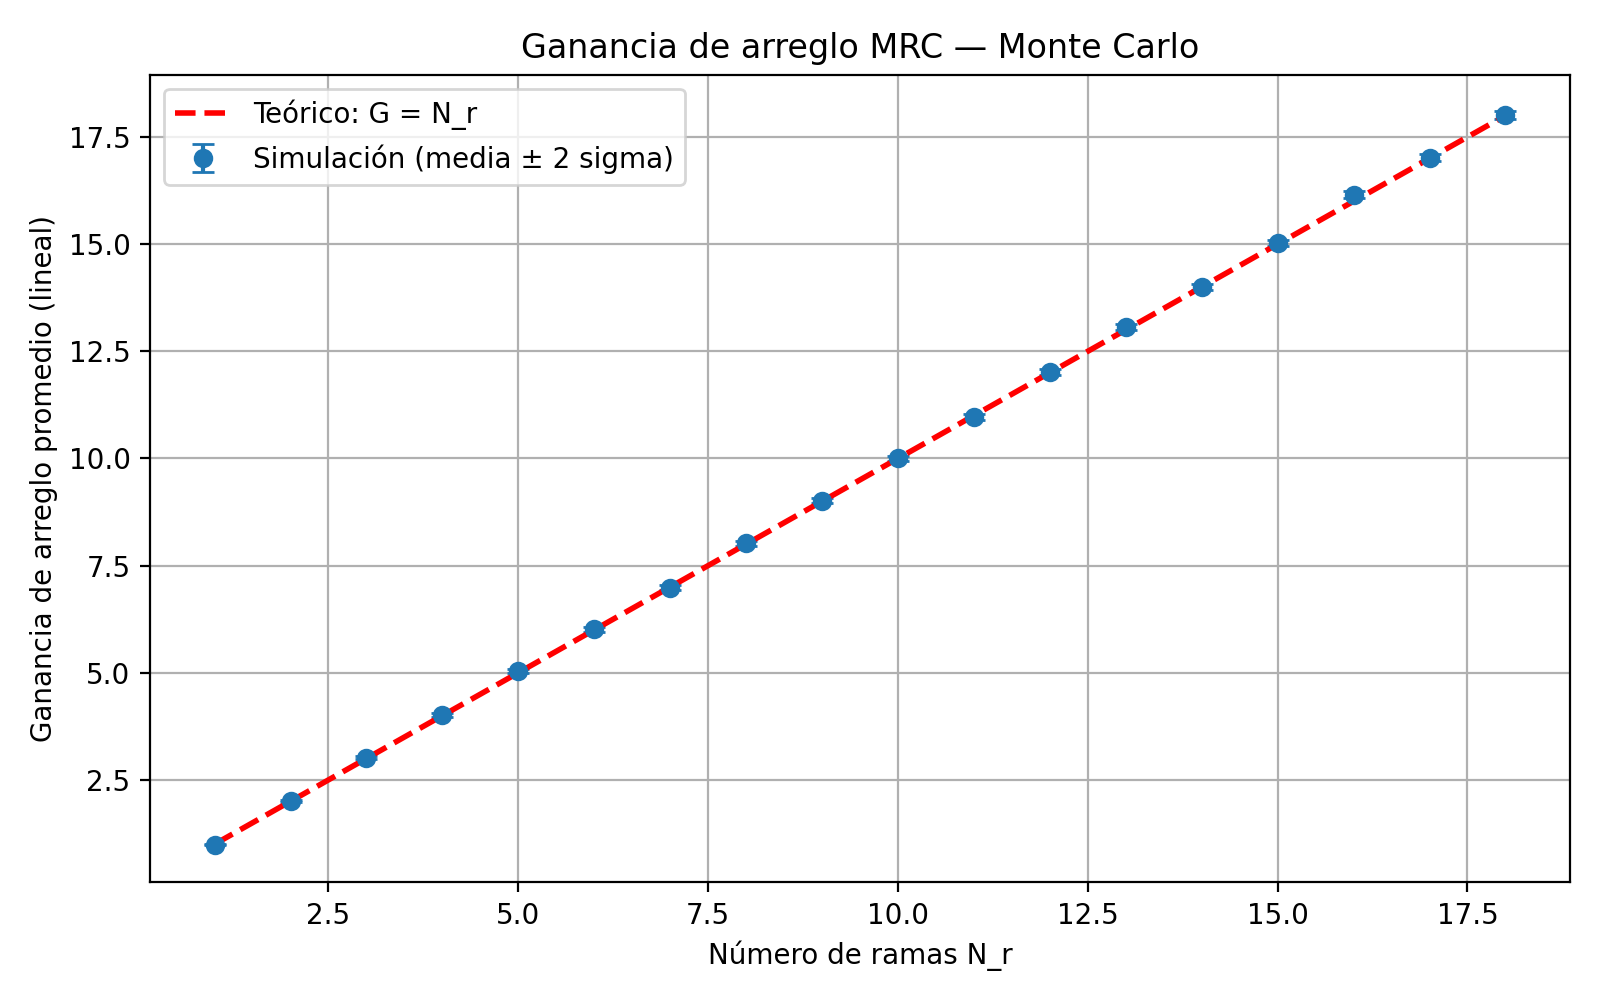
\includegraphics[width=0.8\textwidth]{ganancia_lineal.png}
    \caption{Ganancia de arreglo promedio del combinador MRC en escala lineal.}
    \label{fig:ganancia_lineal}
\end{figure}

Los resultados muestran una coincidencia excelente entre la simulación y la teoría, con errores inferiores al 1\%.  
Esto confirma que la ganancia de arreglo promedio crece linealmente con el número de ramas, tal como predice
\[
\mathbb{E}[G] = N_r, \qquad G_{\text{dB}} = 10 \log_{10}(N_r).
\]

\subsection*{Código}

\lstinputlisting[
    style=mystyle,
    language=Python,
    caption={Archivo \texttt{pregunta20.py}: simulación Monte Carlo del combinador MRC.}
]{pregunta20.py}

\end{document}
